%
\documentclass[8pt]{beamer}


\mode<presentation>
{
  \usetheme{Warsaw}
  \setbeamercovered{invisible}
}
\expandafter\def\expandafter\insertshorttitle\expandafter{%
 \insertshorttitle\hfill%
 \insertframenumber\,/\,\inserttotalframenumber}

% Remove Navigation Symbols
\usenavigationsymbolstemplate{}


%\usepackage{times}
\usepackage[english]{babel}

%\usepackage[latin1]{inputenc}
\usepackage{graphicx}
\usepackage{media9}
    \usepackage[all]{xy}
    \usepackage{xypic}
  \usepackage{times}
    \usepackage{ulem}
    \usepackage[T1]{fontenc}
    \usepackage{amsfonts,amsmath,amssymb}
    \usepackage{hyperref}
    %\usepackage[all]{xy}
    \usepackage{amssymb,amsthm,amsxtra}
    %\usepackage[usenames]{color}
    \usepackage{amscd}
    \usepackage{amsthm}
    \usepackage{amsfonts}
    \usepackage{amssymb}
    \usepackage{mathrsfs}
    \usepackage{mathdots}
%\usepackage{caption} % beamer defines \caption
%\usepackage{subcaption} % this fails to compile with texlive.  We don't really need figure captions in a presentation.  The "readers" don't need to know the exact parameters and all that like in the paper.
\usepackage{verbatim}

\newtheorem*{proposition}{Proposition}
\newtheorem*{prop}{Proposition}
\newtheorem*{remark}{Remark}
\newtheorem*{rem}{Remark}
\newtheorem*{question}{Question}


%\newtheorem*{example}{Example}
%\newtheorem*{theorem}{Theorem}
%\newtheorem*{definition}{Definition}
\newtheorem*{notation}{Notation}
%\newtheorem*{result}{Result}
%\newtheorem*{property}{}
%\newtheorem*{corollary}{Corollary}
%\newtheorem*{construction}{Construction}
%\newtheorem*{case}{Case}
\newtheorem*{conjecture}{Conjecture}
\newtheorem*{setting}{Setting}
\newtheorem*{flowchart}{Flowgausschart}

%\newtheorem{cor}[lemma]{Corollary}
%\newtheorem{exm}[lemma]{Example}
%\newtheorem{exc}[lemma]{Exercise}
%\newtheorem{conj}[lemma]{Conjecture}
%\newtheorem{rem}[lemma]{Remark}
%\newtheorem{conc}[lemma]{Conclusion}


\definecolor{DarkGreen}{rgb}{0,0.5,0}

\begin{document}

\title{Multilevel Aggregation for Image Segmentation}
\author[]{Rachel Tutmaher, James Folberth, and Nathan  Heavner\\}

\date{April 27, 2015}

\begin{frame}
\titlepage
\end{frame}

\begin{frame}
\frametitle{What is Image Segmentation?}
\begin{itemize}
\item Process of subdividing an image into aggregates, aka "salient" segments.
\item Use algorithms to automate the location, classification, or tracking of specific objects within the original image.
\item Each of the pixels in a region that has been deemed "salient" should have similar properties; e.g. color, intensity, texture.
\item Examples: Object Detection, Recognition Tasks, Medical Imaging.
\end{itemize}

\begin{figure}
\centering
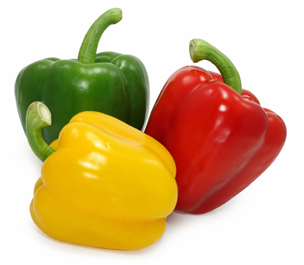
\includegraphics[width=0.4\textwidth,height=0.4\textwidth]{peppers_original.jpg} \hspace{.45cm}
\end{figure}
\end{frame}

\begin{frame}
\frametitle{``Multilevel Space-Time Aggregation for Bright Field Cell Microscopy Segmentation and Tracking." \\ { \small Tiffany Inglis, et al. \textit{International Journal of Biomedical Imaging,} Volume 2010, Article ID 582760}
 }
\begin{itemize}
\item Large amounts of data.
\item Cells have two different basic shapes and may be touching or overlapping.
\item Automatic segmentation and tracking of live cells is a difficult task but vital to live cell studies.
\item Bright field microscopy is well-suited for live cell studies; allows for study of cell morphology and internal cell structure and their dynamics.
\end{itemize}

\begin{figure}
\centering
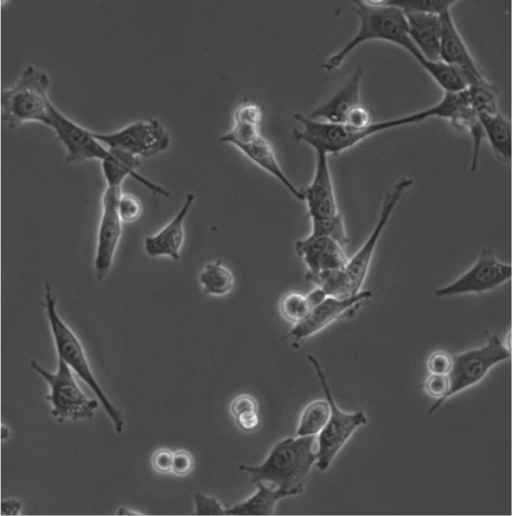
\includegraphics[width=0.4\textwidth,height=0.4\textwidth]{cells.png} \hspace{.45cm}
\end{figure}
\end{frame}

\begin{frame}
\frametitle{Algorithm Description}
\begin{minipage}{.5\textwidth}
\begin{itemize}
\item Each pixel in image is scaled so that maximum intensity value is 1.
\item Problem is analogous to segmentation of a weighted undirected graph: Pixels represent nodes, edge determined by similarity of intensity with neighboring nodes.
\item Edge weights determined by coupling matrix: 
$$ A_{ij} = \left\{ \begin{array}{lr} e^{-\alpha \left| I_i^{[1]}-I_j^{[1]} \right|} & \text{if i, j are neighbors} \\
0 & \text{else} \end{array} \right. $$
\item Pixels recursively grouped: At any point blocks that are sufficiently different from their neighbors are identified as "salient" segments.
\item Stop coarsening when all blocks are "salient"
\item Bottom-up Phase: Uniquely assign all finest-level pixels to one of the segments.
\end{itemize}
\end{minipage}
\hspace{.05\textwidth}
\begin{minipage}{.4\textwidth}
%\begin{figure}
%\centering
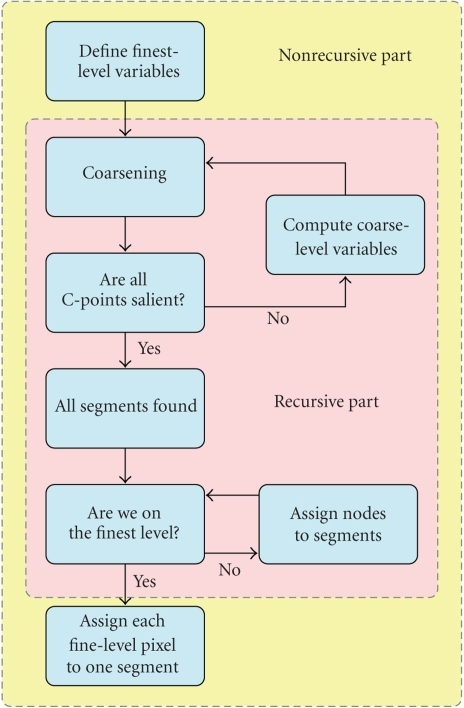
\includegraphics[width=1.2\textwidth]{Flow-Chart.png} \hspace{.45cm}
%\end{figure}
\end{minipage}
\end{frame}

\begin{frame}
\frametitle{Results: Texture Distinction}
\begin{itemize}
\item Initially, weights in the coupling matrix $A$ are based on the average intensity of the block
\item The authors' algorithm scales the weights according to the similarities between two blocks' multilevel variance.
\item This scaling makes it more likely for adjacent blocks with similar textures to be grouped together in subsequent levels.
\end{itemize}

\begin{figure}
\centering

\includegraphics[width=0.2\textwidth,height=0.2\textwidth]{checker_disk_60.png} \hspace{.45cm}

\includegraphics[width=0.2\textwidth,height=0.2\textwidth]{checker_disk_good_seg_1.png} \hspace{.45cm}

\includegraphics[width=0.2\textwidth,height=0.2\textwidth]{checker_disk_good_seg_2.png}
\end{figure}

\end{frame}

\begin{frame}
\frametitle{Results: Scale Invariant Saliency Measure}

\begin{itemize}
\item The saliency measure $\displaystyle{\Gamma_i^{[r]} = \frac{L_{ii}^{[r]}}{(1/2)W_{ii}^{[r]}}}$ can be interpreted as the sum of the coupling coefficients along the border of block $i$ divided by the sum of the coupling coefficients along connections internal to block $i$. 
\item Observe that this saliency measure is neither shape nor scale invariant.
\item The authors make the saliency measure scale invariant by normalizing the weighted boundary length by dividing it by the unweighted boundary length; similarly for the area.
\end{itemize}

\begin{figure}[ht]
\centering

\includegraphics[width=0.15\textwidth,height=0.15\textwidth]{spiral_bad_seg_1.png} \hspace{.45cm}

\includegraphics[width=0.15\textwidth,height=0.15\textwidth]{spiral_bad_seg_2.png} \hspace{.45cm}

\includegraphics[width=0.15\textwidth,height=0.15\textwidth]{spiral_bad_seg_3.png}
~\\Segmentation without scale invariant saliency measure.
\end{figure}
%\vspace{.45cm}

\begin{figure}[ht]
\centering

\includegraphics[width=0.15\textwidth,height=0.15\textwidth]{spiral_good_seg_1.png} \hspace{.45cm}

\includegraphics[width=0.15\textwidth,height=0.15\textwidth]{spiral_good_seg_2.png}
~\\Segmentation with scale invariant saliency measure.
\end{figure}

\end{frame}

\begin{frame}
\frametitle{Results}

\begin{figure}[ht]
\centering
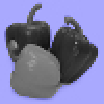
\includegraphics[width=0.2\textwidth,height=0.2\textwidth]{peppers_seg_1.png} \hspace{.45cm}
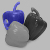
\includegraphics[width=0.2\textwidth,height=0.2\textwidth]{peppers_seg_2.png} \hspace{.45cm}
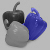
\includegraphics[width=0.2\textwidth,height=0.2\textwidth]{peppers_seg_3.png} \\ \vspace{.45cm}
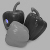
\includegraphics[width=0.2\textwidth,height=0.2\textwidth]{peppers_seg_4.png} \hspace{.45cm}

\includegraphics[width=0.2\textwidth,height=0.2\textwidth]{peppers_seg_5.png}
\end{figure}

\end{frame}


\begin{frame}{Results}
   C. Elegans.

   \begin{figure}[ht]
      \centering
      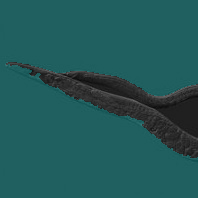
\includegraphics[width=0.3\textwidth]{two_c_elegans_seg_blend_0000.png} \hspace{0.45cm}
      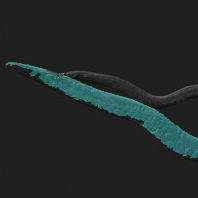
\includegraphics[width=0.3\textwidth]{two_c_elegans_seg_blend_0001.png} \\[0.56cm]
      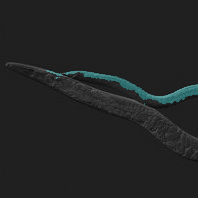
\includegraphics[width=0.3\textwidth]{two_c_elegans_seg_blend_0002.png} \hspace{0.45cm}
      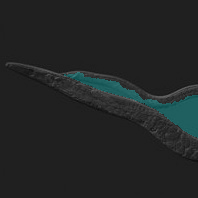
\includegraphics[width=0.3\textwidth]{two_c_elegans_seg_blend_0003.png}
   \end{figure}
\end{frame}


\begin{frame}{Results}
   A pair of overlapping cells.  It appears that one is on top of the other.\\

   \begin{figure}[ht]
      \centering
      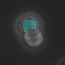
\includegraphics[width=0.3\textwidth]{cells_overlap_seg_blend_0000.png} \hspace{0.45cm}
      
\includegraphics[width=0.3\textwidth]{cells_overlap_seg_blend_0001.png} \hspace{0.45cm}
      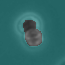
\includegraphics[width=0.3\textwidth]{cells_overlap_seg_blend_0002.png}
   \end{figure}
\end{frame}




\begin{frame}{A few implementation details}
   Our implementation of the segmentation algorithm failed the checkered disk test case!  The authors of the segmentation algorithm specified parameters to use.

   \begin{figure}[ht]
      \centering
      
\includegraphics[width=0.2\textwidth]{checker_disk_60_seg_blend_segAMG_row_sum_0000.png} \hspace{0.45cm}
      
\includegraphics[width=0.2\textwidth]{checker_disk_60_seg_blend_segAMG_row_sum_0001.png} \hspace{0.45cm}
      
\includegraphics[width=0.2\textwidth]{checker_disk_60_seg_blend_segAMG_row_sum_0002.png} \hspace{0.45cm}
      
\includegraphics[width=0.2\textwidth]{checker_disk_60_seg_blend_segAMG_row_sum_0003.png}
      ~\\Inglis coarsener with off-diagonal row sum strengths.
   \end{figure}

   \begin{figure}[ht]
      \centering
      
\includegraphics[width=0.2\textwidth]{checker_disk_60_seg_blend_RSAMG_row_sum_0000.png} \hspace{0.45cm}
      
\includegraphics[width=0.2\textwidth]{checker_disk_60_seg_blend_RSAMG_row_sum_0001.png} 
      ~\\Ruge-St\"uben coarsener with off-diagonal row sum strengths.
   \end{figure}

\end{frame}


\begin{frame}{A few implementation details}
   Our implementation of the segmentation algorithm failed the checkered disk test case!  The authors of the segmentation algorithm specified parameters to use.

   \begin{figure}[ht]
      \centering
      
\includegraphics[width=0.2\textwidth]{checker_disk_60_seg_blend_segAMG_max_el_0000.png} \hspace{0.45cm}
      
\includegraphics[width=0.2\textwidth]{checker_disk_60_seg_blend_segAMG_max_el_0001.png}
      ~\\Inglis coarsener with maximum off-diagonal element strengths.
   \end{figure}

   \begin{figure}[ht]
      \centering
      
\includegraphics[width=0.2\textwidth]{checker_disk_60_seg_blend_RSAMG_row_sum_0000.png} \hspace{0.45cm}
      
\includegraphics[width=0.2\textwidth]{checker_disk_60_seg_blend_RSAMG_row_sum_0001.png} 
      ~\\Ruge-St\"uben coarsener with off-diagonal row sum strengths.
   \end{figure}

\end{frame}




\begin{frame}{A few implementation details}
   The segmentation algorithm uses a graph coarsener that is very similar to Ruge-St\"uben AMG.  The coarsener in RS AMG scales linearly with problem size.  The segmentation algorithm, as written, appears to scale \emph{quadratically} with problem size!\\[0.5cm]

   \begin{minipage}{0.45\textwidth}
      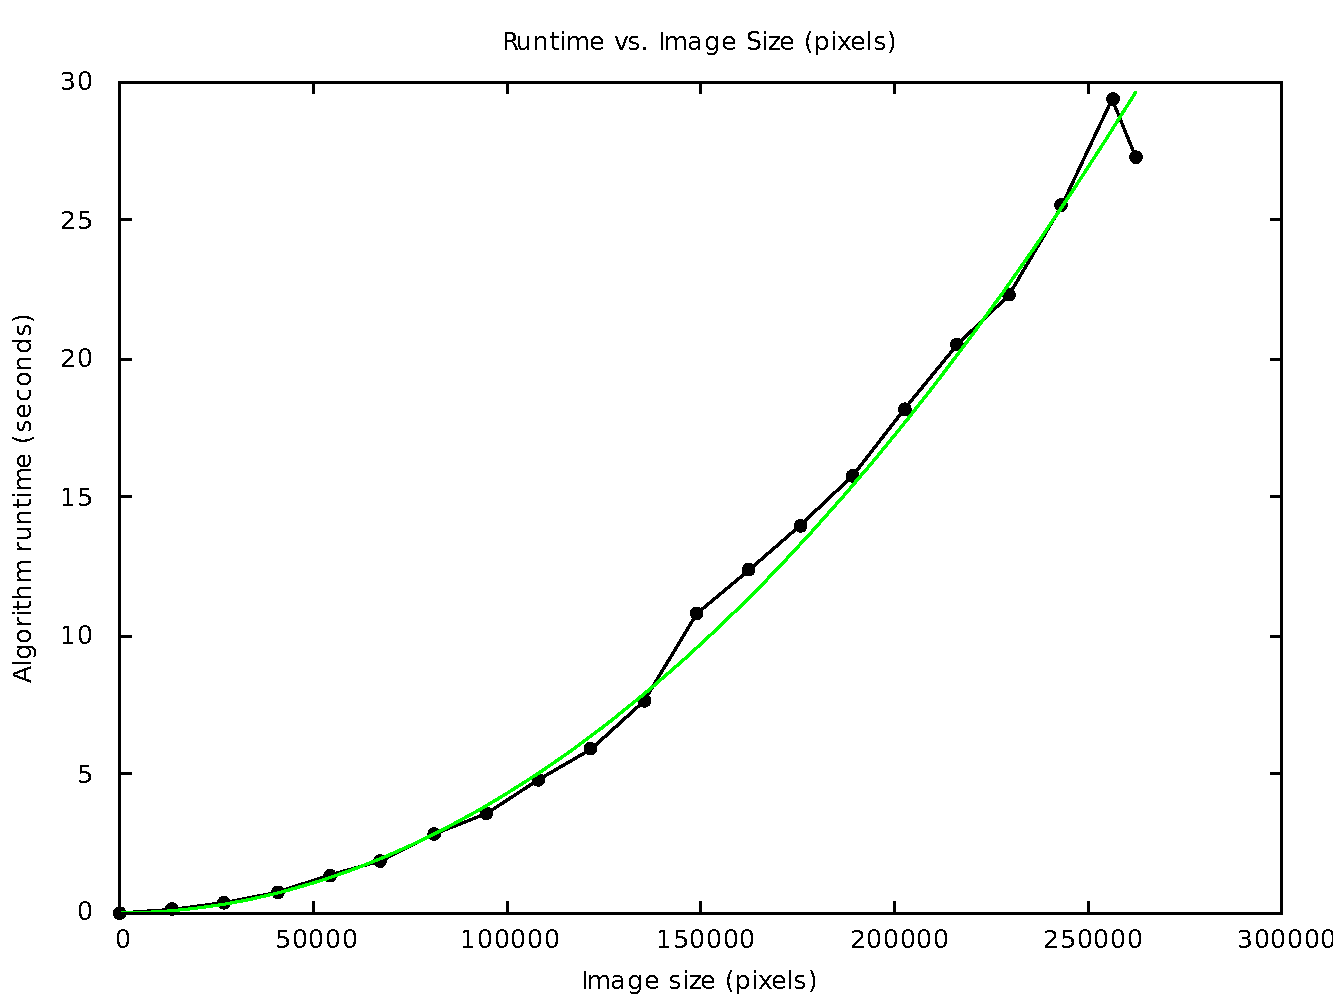
\includegraphics[width=\textwidth]{runtime_scaling_segAMG_spiral_512_james.pdf}
      ~\\Inglis coarsening.
   \end{minipage}
   \hspace{0.05\textwidth}
   \begin{minipage}{0.45\textwidth}
      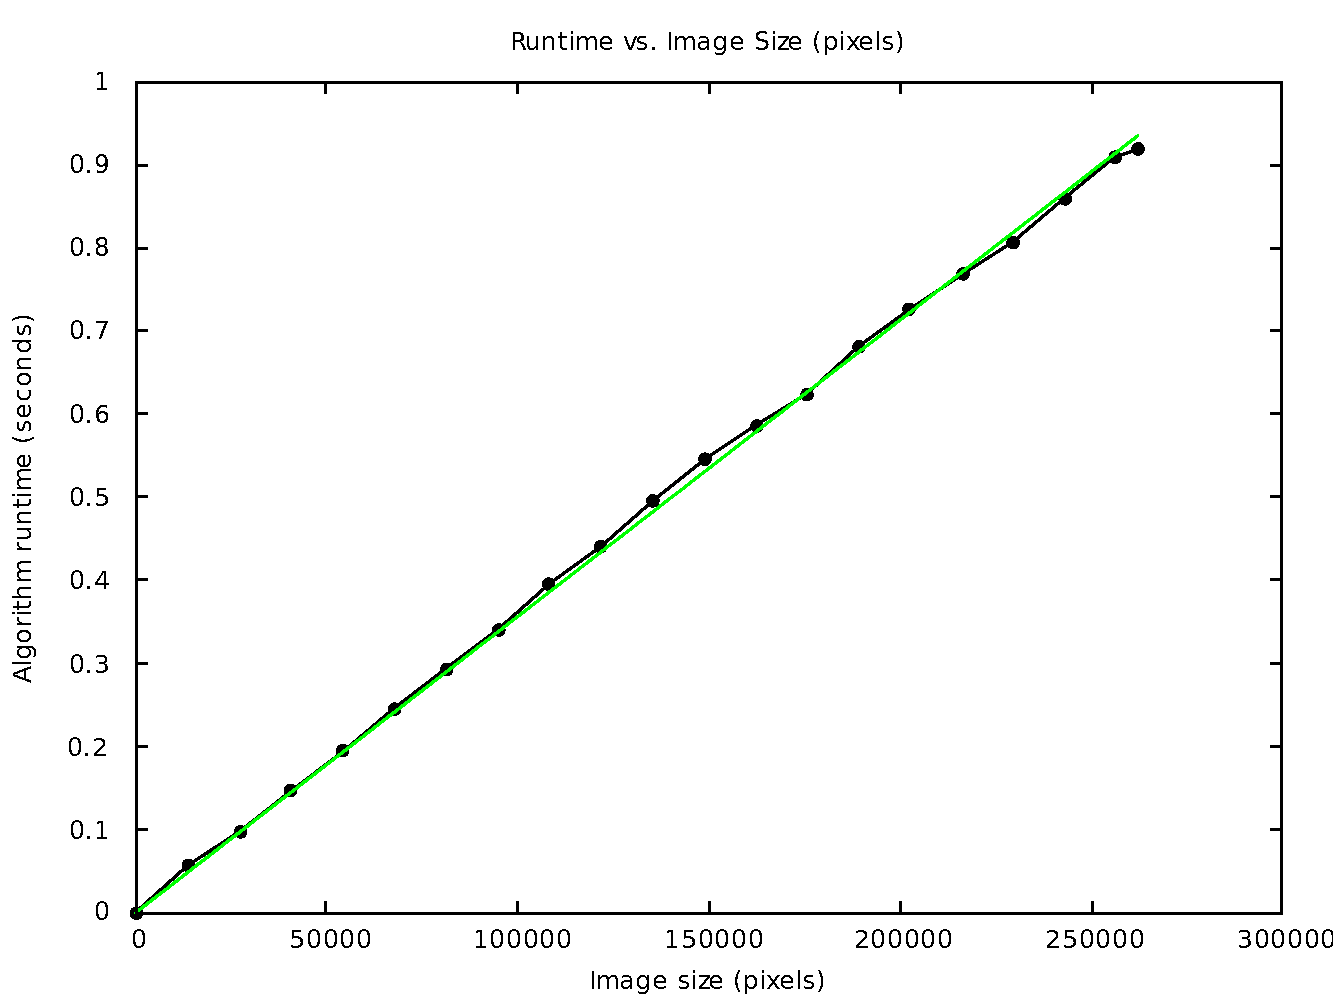
\includegraphics[width=\textwidth]{runtime_scaling_RSAMG_spiral_512_james.pdf}
      ~\\Ruge-St\"uben coarsening.
   \end{minipage}

\end{frame}


\begin{frame}{Questions?}

   Inglis et al., ``Multilevel space-time aggregation for bright field cell microscopy segmentation and tracking'', International Journal of Biomedical Imaging, (2010).\\[1cm]

   Questions?\\[.5cm]

   \begin{minipage}{0.45\textwidth}
      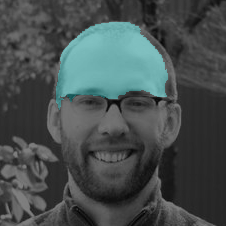
\includegraphics[width=\textwidth]{ck_seg_blend_0001.png} \hspace{0.45cm}
   \end{minipage}
   \hspace{0.05\textwidth}
   \begin{minipage}{0.45\textwidth}
      %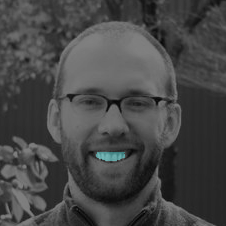
\includegraphics[width=0.4\textwidth]{ck_seg_blend_0006.png}
      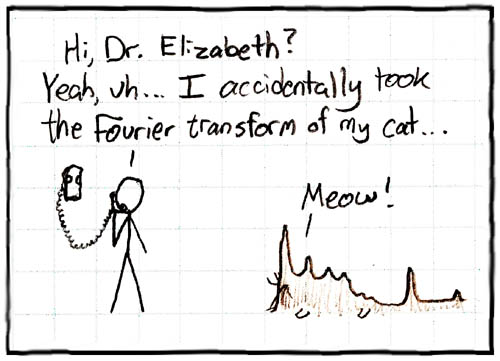
\includegraphics[width=\textwidth]{xkcd_fourier.jpg}\\
      Credit: xkcd.com, \# 26
   \end{minipage}

\end{frame}


%%%%%%%%%%%%%%%%%%%%%% BEGIN COMMENT %%%%%%%%%%%%%%%%%%%%%%%%%%%%%%%%%
\begin{comment}

\title{Numerical Analysis in High Dimensions}
\author[]{ Nathan H., Andrew W., Andrew C., Ryan A., and Jeremiah C.\\ Dr. Pierre Gremaud, Rachael Gordon-Wright }

\begin{frame}
\titlepage
\end{frame}


\begin{frame}
\frametitle{Background}
\begin{itemize}
\item Uncertain parameters in equations  
\item A "solution" of the equation involves probability
\item Two options: Monte Carlo simulations or pdf of the function
\end{itemize}
\begin{figure}
\includegraphics[width=.8\linewidth]{CIex.jpg}
\end{figure}
\end{frame}


\begin{frame}
\frametitle{Outline}
\begin{itemize}
\item Description of sample problem
\vspace{4mm}
\item Our method: deriving and solving the pdf equation
\vspace{4mm}
\item "Old" method: Monte Carlo simulations
\vspace{4mm}
\item Discussion of results
\vspace{4mm}
\item Applying this method to other equations
\vspace{4mm}
\item Future work
\end{itemize}
\end{frame}

\begin{frame}
\frametitle{Sample Problem} 
\begin{itemize} 
\item Van der Pol equation
		\begin{itemize} 
		\item $\frac{d^2u}{dt} - \mu(1-u^2) \frac{du}{dt} + u = 0$ 
			\begin{itemize}
			\item $\mu$ is a parameter, describes strength of oscillations
			\end{itemize}
		\item Solve by splitting it up into two first-order ODEs
			\begin{itemize}
			\item $\frac{du}{dt} = v$
			\item $\frac{dv}{dt} - \mu(1-u^2) + u = 0$
			\end{itemize}
		\end{itemize} 
\item Initial conditions 
	\begin{itemize} 
	\item $u(0) = 1 + \eta$ 
	\item $v(0) = \zeta$ 
	\item $\eta, \zeta \sim \mathcal{N}(0,0.01)$
	\end{itemize}
\item Resolution of problem 
	\begin{itemize} 
	\item Stochastic initial conditions: Statistical approach 
	\item Probability Density Function: p(X) = P(x=X)
	\item Nonlinear system: Numerical approach
	\end{itemize}
\end{itemize}
\end{frame}
	
\begin{frame}

	\frametitle{Deriving the PDF equation for the Van der Pol Oscillator}
	\begin{itemize}

	\item We define the raw PDF function as:
	\begin{equation}
	\Pi = \delta(U-u(t))\delta(V-v(t)),
	\end{equation}
	where E[\textit{$\Pi$}] = p(U,V,t) (PDF function).
	\vspace{3 mm}
	
	\item We multiply \textit{$\frac{du}{dt}$} by \textit{$\frac{\partial\Pi}{\partial U}$}, and \textit{$\frac{dv}{dt}$} by \textit{$\frac{\partial\Pi}{\partial V}$} in order to get following equation:
	\begin{equation}
	\frac{\partial\Pi}{\partial t} + V\frac{\partial\Pi}{\partial U} + [\mu(1 - U^2)V-U]\frac{\partial\Pi}{\partial V} = 0
	\end{equation}

	\vspace{3 mm}
	\item Taking the expected value of both sides leads to the PDF equation:
	\begin{equation}
	\frac{\partial p}{\partial t} + V\frac{\partial p}{\partial U} + [\mu(1 - U^2)V-U]\frac{\partial p}{\partial V} = 0
	\end{equation}	

	\end{itemize}
\end{frame}

\begin{frame}
\frametitle{Results: PDE vs. Monte-Carlo}
\begin{figure}
\includegraphics[width=1\linewidth]{comparison_1.eps}
\caption{mu = 0.5}
\end{figure}
\end{frame}

\begin{frame}
\frametitle{Results: PDE vs. Monte-Carlo}
\begin{figure}
\includegraphics[width=1\linewidth]{comparison_2.eps}
\caption{mu = 1.5}
\end{figure}
\end{frame}

\begin{frame}
\frametitle{Results: PDE vs. Monte-Carlo}
\begin{figure}
\includegraphics[width=1\linewidth]{comparison_3.eps}
\caption{mu = 5}
\end{figure}
\end{frame}

\begin{frame}
\frametitle{Wave Equation}
\begin{itemize}
\item Standard Form
\begin{itemize}
\item $\frac{\partial^2 u}{\partial t^2}-c^2\frac{\partial^2 u}{\partial x^2} = 0$
\item u(x,t) = amplitude of wave
\item c = speed of propagation
\end{itemize}
\item First Order System
\begin{itemize}
\item Let $u_1 = \frac{\partial u}{\partial t}$ and $u_2 = \frac{\partial u}{\partial x}$
\item $\frac{\partial u_1}{\partial t} - c^2 \frac{\partial u_2}{\partial x} = 0$
\item $\frac{\partial u_2}{\partial t} - \frac{\partial u_1}{\partial x} = 0$
\end{itemize}
\item Analytical Solution to First Order PDEs (Advection Equations)
\begin{itemize}
\item If $\frac{\partial u}{\partial t} - c \frac{\partial u}{\partial x} = 0$
\item $u(x,t) = u_0(x-ct)$
\end{itemize}
\end{itemize}
\end{frame}

\begin{frame}
\frametitle{Sample Problem}
\begin{itemize}
\item System
\begin{itemize}
\item $\frac{\partial u_1}{\partial t} - c^2 \frac{\partial u_2}{\partial x} = 0$
\item $\frac{\partial u_2}{\partial t} - \frac{\partial u_1}{\partial x} = 0$
\item $c \sim \mathcal{U}(1-\epsilon,1+\epsilon)$
\end{itemize}
\item $2\pi$-periodic boundary conditions
\item Initial conditions
\begin{itemize}
\item $u_1(x,0) = sin(x) + \eta$
\item $u_2(x,0) = cos(x) + \zeta$
\item $\eta, \zeta \sim \mathcal{N}(0,1)$
\end{itemize}
\item Computing the CDF
\begin{itemize}
\item Analytical CDF
\begin{itemize}
\item Only for deterministic speeds $(\epsilon = 0)$
\end{itemize}
\item Monte Carlo simulation
\item Our derivation of the PDF/CDF
\begin{itemize}
\item Error from calculating expected values (closure rules)
\item Error from discretization
\end{itemize}
\end{itemize}
\end{itemize}
\end{frame}

\begin{frame}
\frametitle{Results}
\begin{figure}
\centering
\begin{subfigure}{.5\textwidth}
\centering
\includegraphics[width=1\linewidth]{cdf_ana_wave.eps}
\caption{Monte Carlo approximation to CDF}
\end{subfigure}%
\begin{subfigure}{.5\textwidth}
\centering
\includegraphics[width=1\linewidth]{cdf_num_wave.eps}
\caption{Numerical approximation to CDF}
\end{subfigure}
\end{figure}
\end{frame}

\begin{frame}
\frametitle{Future Steps and Applications}

\begin{columns}

\begin{column}{0.5 \textwidth}
\begin{itemize}
\setlength{\itemsep}{5pt}

\item Previously mentioned issues

\item Expand method to a broader range of problems: 
	\begin{itemize}
	\setlength{\itemsep}{2pt}
	\item Lorenz equations model atmospheric convection, and are very sensitive to initial conditions. 
		$$\left\{\begin{array}{l}
		\displaystyle{\frac{dx}{dt} = \sigma (y - x)} \\ \\
		\displaystyle{\frac{dy}{dt} = x(\rho - z) - y} \\ \\
		\displaystyle{\frac{dz}{dt} = xy - \beta z}\end{array}\right.$$
		
	\item Other ODEs 
	\item PDEs (wave and acoustic wave equations, specifically)	\end{itemize}
\end{itemize}

\end{column}

\begin{column}{0.5 \textwidth}
\begin{figure}

\includegraphics[width = 2in]{lorenz_attractor.png}
\caption{The Lorenz Butterfly}

\end{figure}
\end{column}

\end{columns}

\end{frame}

\begin{frame}

\frametitle{Method of Lines}

\begin{columns}

\begin{column}{0.5 \textwidth}
\begin{itemize}

\item Use semi-discretization (method of lines) to estimate the pdf of a stochastic partial differential equation.

	\begin{itemize} 
	\setlength{\itemsep}{2pt}
	\item $\displaystyle{\frac{du_i}{dt} = \mathfrak{F}(u_{i-1}, u_i, u_{i+1})}$
	\item Each differential equation represents a node of the discretization
	\item Number of dimensions increases quickly
	\end{itemize}

\end{itemize}

\end{column}

\begin{column}{0.5 \textwidth}
\begin{figure}

\includegraphics[width = 2in]{MOL.png}
\caption{Method of Lines for a heat problem}

\end{figure}
\end{column}
\end{columns}
\end{frame}

\begin{frame}
\frametitle{Acknowledgments}
\begin{itemize}
\item National Science Foundation grant numbers DMS-1063010 and DMS-0943855
\item National Security Agency grant number H98230-12-0299
\item Faculty mentor: Dr. Pierre Gremaud
\item Graduate mentor: Rachael Gordon-Wright
\end{itemize}
\end{frame}

\end{comment}
%%%%%%%%%%%%%%%%%%%%%%% END COMMENT %%%%%%%%%%%%%%%%%%%%%%%%%%%%%%%


\end{document}
